\documentclass[11pt,a4paper]{article}

\usepackage[utf8]{inputenc}
\usepackage[T1]{fontenc}
\usepackage[a4paper,margin=2.5cm]{geometry}
\usepackage{amsmath,amssymb}
\usepackage{graphicx}
\usepackage{booktabs}
\usepackage{enumitem}
\usepackage{hyperref}
\usepackage{xcolor}
\usepackage{fancyhdr}
\usepackage{titlesec}

\hypersetup{
  colorlinks=true,
  linkcolor=blue!50!black,
  citecolor=blue!50!black,
  urlcolor=blue!50!black
}

\titleformat{\section}{\normalfont\Large\bfseries}{\thesection}{1em}{}
\titleformat{\subsection}{\normalfont\large\bfseries}{\thesubsection}{1em}{}

\pagestyle{fancy}
\fancyhf{}
\rhead{\small Résumé d'article --- SVD}
\lhead{\small Hippolyte Perraud}
\cfoot{\thepage}

\newcommand{\R}{\mathbb{R}}
\newcommand{\C}{\mathbb{C}}

\title{\vspace{-1.5cm}\textbf{La Décomposition en Valeurs Singulières (SVD)\\
\large Fondements mathématiques, propriétés et applications}}
\author{Hippolyte Perraud \\ \small INSA Rouen Normandie -- Département Mathématiques Appliquées}
\date{\today}

\begin{document}

\maketitle
\thispagestyle{fancy}

\begin{abstract}
\noindent Ce document propose un résumé structuré du premier chapitre de l'ouvrage \emph{Data-Driven Science and Engineering} de S. L. Brunton et J. N. Kutz, consacré à la décomposition en valeurs singulières (SVD). Après avoir rappelé la définition et les propriétés mathématiques fondamentales de cette factorisation matricielle, on présente ses principales applications : approximation de matrices de rang faible, calcul de pseudo-inverse et régression, analyse en composantes principales, avant de discuter des questions pratiques de troncature et des extensions modernes (SVD randomisée, décompositions tensorielles).
\end{abstract}

\vspace{0.3cm}

\section{Introduction}

La décomposition en valeurs singulières (SVD, pour \emph{Singular Value Decomposition}) est l'une des factorisations matricielles les plus utilisées en science des données. Contrairement à la décomposition en valeurs propres, elle existe pour \emph{toute} matrice, y compris rectangulaire, ce qui en fait un outil universel et numériquement stable. Elle sert de brique de base à un grand nombre de méthodes présentées comme fondamentales en apprentissage automatique et en calcul scientifique : approximation de rang faible, analyse en composantes principales (PCA), pseudo-inverse pour la résolution de systèmes linéaires, décomposition en modes dynamiques (DMD) ou décomposition orthogonale aux valeurs propres (POD).

L'idée centrale est la suivante : de nombreux jeux de données de grande dimension (images, vidéos, mesures physiques, séries temporelles) possèdent en réalité une structure de rang faible, c'est-à-dire qu'un petit nombre de motifs dominants suffit à expliquer l'essentiel de la variabilité observée. La SVD fournit un moyen systématique, purement piloté par les données, d'extraire ces motifs. En ce sens, elle peut être vue comme une généralisation de la transformée de Fourier rapide (FFT) : alors que la FFT projette les données sur une base fixe et générique (sinusoïdes), la SVD construit une base \emph{adaptée aux données elles-mêmes}.

\section{Définition et construction de la SVD}

\subsection{Formulation générale}

Soit une matrice de données $X \in \C^{n \times m}$, dont les colonnes $x_k$ (appelées \emph{snapshots}) représentent par exemple des mesures successives d'un système physique, des images vectorisées, ou des observations statistiques. La SVD de $X$ s'écrit :
\begin{equation}
X = U \Sigma V^{*},
\end{equation}
où $U \in \C^{n\times n}$ et $V \in \C^{m \times m}$ sont des matrices \emph{unitaires} ($UU^{*}=U^{*}U=I$), et $\Sigma \in \R^{n \times m}$ est une matrice diagonale à coefficients réels positifs ou nuls, rangés par ordre décroissant. Les colonnes de $U$ sont appelées \emph{vecteurs singuliers gauches}, celles de $V$ \emph{vecteurs singuliers droits}, et les coefficients diagonaux de $\Sigma$ les \emph{valeurs singulières}. Le rang de $X$ est égal au nombre de valeurs singulières non nulles. L'existence de cette décomposition est garantie pour toute matrice complexe, contrairement à la décomposition spectrale qui exige des conditions sur la matrice (carrée, diagonalisable).

\subsection{SVD complète et SVD économique}

Lorsque $n \geq m$, au plus $m$ valeurs singulières sont non nulles. On peut alors écrire une version réduite, dite \emph{économique}, en ne conservant que les $m$ premières colonnes de $U$ (notées $\hat U$) et le bloc utile de $\Sigma$ (noté $\hat \Sigma$) :
\begin{equation}
X = \hat U \hat \Sigma V^{*}.
\end{equation}
Les colonnes de $\hat U$ forment une base orthonormée de l'espace des colonnes (\emph{column space}) de $X$, tandis que le complément orthogonal $\hat U_{\perp}$ n'intervient pas dans la reconstruction exacte de $X$. Cette version économique est nettement plus efficace en mémoire et en temps de calcul lorsque $X$ est très rectangulaire.

D'un point de vue numérique, le calcul de la SVD est aujourd'hui une opération mature, disponible nativement dans la plupart des environnements scientifiques (\texttt{svd} en Matlab et R, \texttt{numpy.linalg.svd} en Python), et implémentée en interne via la routine \texttt{DGESVD} de la bibliothèque LAPACK. L'origine théorique de la SVD remonte aux travaux de Beltrami et Jordan (1873), Sylvester (1889), Schmidt (1907) puis Weyl (1912) ; les algorithmes numériques modernes doivent beaucoup aux travaux de Golub à partir des années 1960.

\section{Propriétés mathématiques fondamentales}

\subsection{Lien avec les matrices de corrélation}

La SVD entretient un lien étroit avec les matrices de corrélation $XX^{*}$ et $X^{*}X$. En injectant $X = U\Sigma V^{*}$, on montre que :
\begin{align}
XX^{*} &= U \begin{bmatrix} \hat\Sigma^2 & 0 \\ 0 & 0 \end{bmatrix} U^{*}, &
X^{*}X &= V \hat\Sigma^2 V^{*}.
\end{align}
Autrement dit, les colonnes de $U$ sont les vecteurs propres de $XX^{*}$, celles de $V$ sont les vecteurs propres de $X^{*}X$, et les valeurs singulières non nulles sont les racines carrées des valeurs propres (communes) de ces deux matrices de corrélation. Cette observation est à la base de la \emph{méthode des snapshots} (Sirovich, 1987) : lorsque la dimension $n$ est trop grande pour diagonaliser $XX^{*}$ directement, il est possible de résoudre le problème aux valeurs propres, plus petit, sur $X^{*}X$, puis de reconstruire les vecteurs singuliers gauches manquants par $\hat U = X \hat V \hat \Sigma^{-1}$.

\subsection{Interprétation géométrique}

Géométriquement, la matrice $X$ transforme la sphère unité de $\R^n$ en un ellipsoïde de $\R^m$ (figure~\ref{fig:geom}) : les directions principales de cet ellipsoïde sont données par les colonnes de $U$, et leurs longueurs par les valeurs singulières correspondantes, tandis que les colonnes de $V$ indiquent les directions de l'espace de départ qui se transforment en ces axes principaux. Cette lecture géométrique explique pourquoi la SVD caractérise si naturellement la géométrie d'une application linéaire entre deux espaces vectoriels.

\begin{figure}[h]
\centering
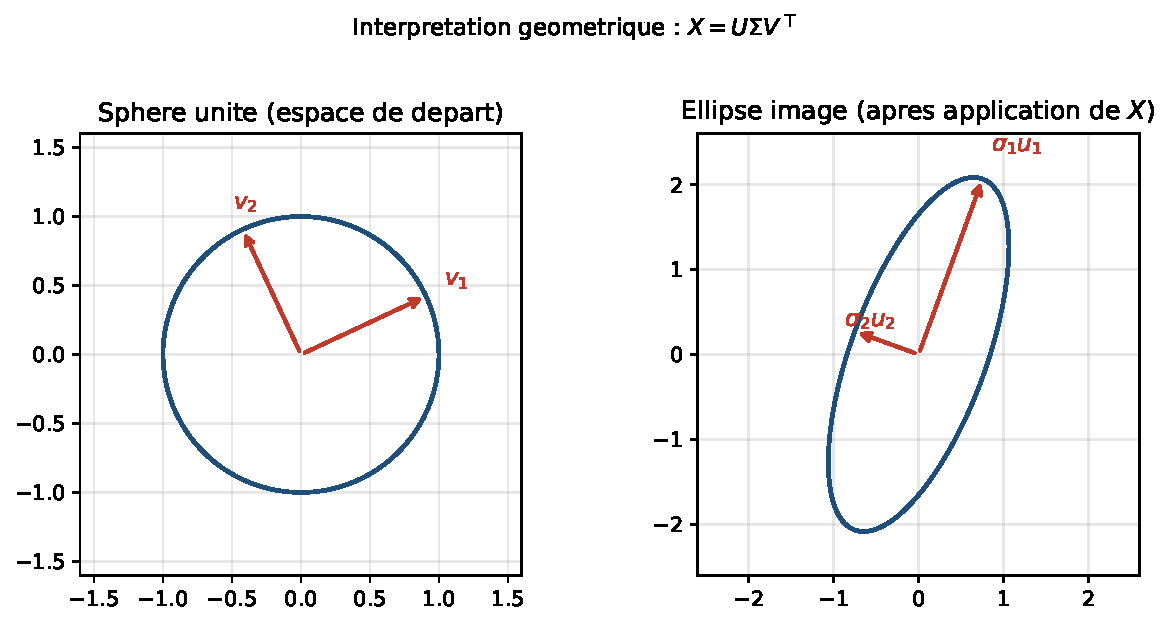
\includegraphics[width=0.85\textwidth]{figures/geometrie.pdf}
\caption{Illustration schématique (cas $2\times 2$) : la SVD décrit comment une matrice $X$ transforme la sphère unité en un ellipsoïde dont les demi-axes sont les valeurs singulières $\sigma_i$, orientés selon les vecteurs singuliers gauches $u_i$.}
\label{fig:geom}
\end{figure}

\subsection{Invariance aux transformations unitaires}

Une propriété remarquable de la SVD est son invariance vis-à-vis des transformations unitaires : si l'on multiplie $X$ à gauche (respectivement à droite) par une matrice unitaire $C$ (resp. $P^{*}$), seule la matrice $U$ (resp. $V$) est modifiée, tandis que les valeurs singulières restent inchangées. Cette propriété a une conséquence pratique importante : comme la transformée de Fourier discrète est elle-même une transformation unitaire, la SVD de données transformées par Fourier possède exactement le même spectre de valeurs singulières que la SVD des données originales.

\section{Approximation de rang faible et théorème d'Eckart--Young}

La propriété sans doute la plus utile de la SVD est de fournir, pour tout rang $r$, la meilleure approximation possible de $X$ par une matrice de rang $r$, au sens de la norme de Frobenius. C'est le contenu du théorème d'Eckart--Young (généralisation par Schmidt d'un résultat sur les espaces fonctionnels, redécouvert par Eckart et Young en 1936) :
\begin{equation}
\underset{\tilde X,\ \mathrm{rang}(\tilde X)=r}{\arg\min} \ \| X - \tilde X \|_F = \tilde U \tilde \Sigma \tilde V^{*},
\end{equation}
où $\tilde U, \tilde V$ regroupent les $r$ premières colonnes de $U$ et $V$, et $\tilde \Sigma$ le bloc $r\times r$ correspondant de $\Sigma$. De façon équivalente, l'approximation optimale de rang $r$ s'écrit comme une somme de $r$ matrices de rang 1 (décomposition dyadique) :
\begin{equation}
\tilde X = \sum_{k=1}^{r} \sigma_k u_k v_k^{*}.
\end{equation}
Ce résultat a une portée considérable : il garantit qu'aucune autre méthode ne peut produire, pour un rang fixé, une approximation plus fidèle que la troncature de la SVD. De plus, la hiérarchie des approximations est \emph{emboîtée} : les $r$ premiers modes de la solution de rang $r$ sont exactement les $r$ premiers modes de la solution de rang $r+1$, ce qui permet de faire varier $r$ sans recalculer la décomposition.

\subsection{Illustration : compression d'image}

L'exemple canonique de cette propriété est la compression d'images. Une image en niveaux de gris peut être vue comme une matrice $X \in \R^{n\times m}$ dont les lignes et colonnes correspondent aux pixels. En ne conservant que les $r$ premiers termes de la décomposition dyadique, on obtient une image approchée qui ne nécessite de stocker que $r(n+m+1)$ valeurs au lieu de $nm$. Sur l'exemple présenté dans l'ouvrage (image de $2000\times 1500$ pixels), une troncature à $r=100$ suffit déjà à obtenir une image visuellement fidèle, alors que cela ne représente qu'environ $11\,\%$ de l'espace de stockage original ; les valeurs singulières décroissent en effet très rapidement, si bien que les cent premiers modes concentrent déjà près de $80\,\%$ de l'énergie totale (figure~\ref{fig:singvals}, illustration schématique avec des données synthétiques reproduisant cette décroissance typique).

\begin{figure}[h]
\centering
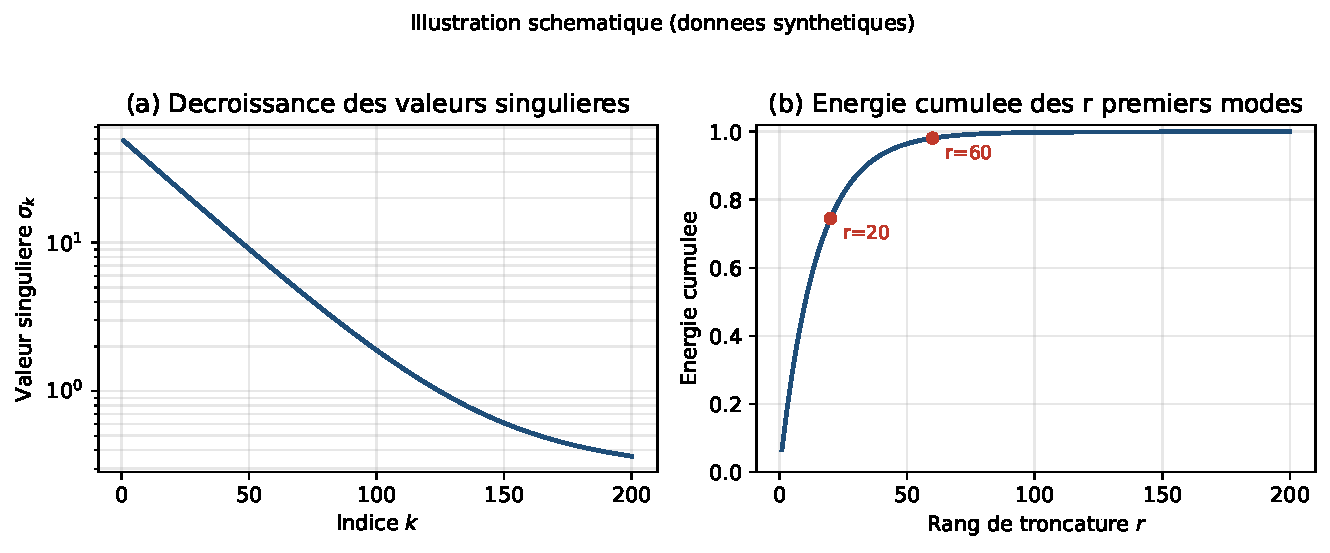
\includegraphics[width=\textwidth]{figures/singvals.pdf}
\caption{Décroissance typique des valeurs singulières (a) et énergie cumulée en fonction du rang de troncature $r$ (b). Plus la décroissance est rapide, plus une approximation de rang faible est pertinente.}
\label{fig:singvals}
\end{figure}

\section{Pseudo-inverse, moindres carrés et régression}

La SVD est l'outil de référence pour résoudre les systèmes linéaires $Ax=b$ lorsque $A$ n'est ni carrée ni inversible. Deux cas se présentent : si $A$ est \emph{sous-déterminée} (plus de colonnes que de lignes), il existe généralement une infinité de solutions et l'on cherche celle de norme minimale ; si $A$ est \emph{sur-déterminée} (plus de lignes que de colonnes), il n'existe généralement pas de solution exacte, et l'on cherche celle qui minimise l'erreur quadratique $\|Ax-b\|_2$ (solution des moindres carrés). Ces deux problèmes se résolvent au moyen du \emph{pseudo-inverse de Moore-Penrose} :
\begin{equation}
A^{\dagger} \triangleq \tilde V \tilde \Sigma^{-1} \tilde U^{*}, \qquad \tilde x = A^{\dagger} b = \tilde V \tilde \Sigma^{-1} \tilde U^{*} b.
\end{equation}
Ce calcul est particulièrement efficace : l'inversion des matrices unitaires $\tilde U$ et $\tilde V$ revient à une simple transposition ($\mathcal O(n^2)$), et $\tilde \Sigma$ étant diagonale, son inversion coûte $\mathcal O(n)$, contre $\mathcal O(n^3)$ pour l'inversion générique d'une matrice dense. L'ouvrage illustre cette approche sur des cas concrets : régression linéaire à une variable (ajustement d'une pente à partir de données bruitées), puis régression multilinéaire sur deux jeux de données réels (composition de mélanges de ciment et production de chaleur ; caractéristiques du marché immobilier de Boston), montrant que la SVD fournit directement les coefficients de régression au sens des moindres carrés.

\section{Analyse en composantes principales (PCA)}

L'analyse en composantes principales, développée indépendamment par Pearson (1901) puis Hotelling (1930), peut être vue comme une application directe de la SVD. Le principe consiste à centrer les données (soustraction de la moyenne ligne par ligne) puis à calculer la SVD de la matrice centrée $B = X - \bar X$. Les composantes principales sont alors les vecteurs singuliers gauches de $B$, hiérarchisés par la quantité de variance qu'ils expliquent ; la matrice de covariance $C = \tfrac{1}{n-1}B^{*}B$ admet exactement cette même base de vecteurs propres. La SVD offre ainsi une alternative numériquement plus stable au calcul direct de la matrice de covariance et de sa diagonalisation.

\subsection{Exemple : les \emph{eigenfaces}}

L'une des illustrations les plus marquantes de la PCA est le problème des \emph{eigenfaces} (Sirovich et Kirby, 1987 ; Turk et Pentland, 1991). Une bibliothèque de visages, soigneusement recadrés et alignés, est vectorisée puis centrée ; la SVD de la matrice résultante fournit un ensemble de « visages propres » qui forment une base adaptée à la représentation des visages humains. Un visage absent de l'échantillon d'apprentissage peut alors être approché par projection sur les $r$ premiers eigenfaces ; sur l'exemple étudié, la reconstruction reste grossière pour $r \le 200$ mais devient satisfaisante au-delà de $r \approx 400$, sur un espace image de plus de $32\,000$ dimensions. Au-delà de la compression, cette représentation possède une propriété essentielle pour la reconnaissance : les images d'un même individu, projetées sur quelques composantes principales bien choisies, forment des groupes (\emph{clusters}) bien séparés dans cet espace réduit, ce qui constitue la base de nombreuses méthodes de classification d'images.

\section{Choix de la troncature et limites de la méthode}

\subsection{Seuillage optimal des valeurs singulières}

Le choix du rang de troncature $r$ reste l'une des décisions les plus délicates en pratique. L'approche la plus simple consiste à fixer un seuil sur l'énergie cumulée (par exemple $90\,\%$ ou $99\,\%$ de la variance totale), mais cette règle reste arbitraire. Gavish et Donoho (2014) proposent une approche plus rigoureuse : en supposant que la matrice observée est la somme d'une matrice de rang faible et d'un bruit blanc gaussien d'amplitude $\gamma$, il existe un seuil dur optimal $\tau$ au-delà duquel toute valeur singulière doit être conservée. Pour une matrice carrée, ce seuil vaut $\tau = (4/\sqrt3)\sqrt n\,\gamma$ ; pour une matrice rectangulaire de rapport d'aspect $\beta = m/n$, la constante $4/\sqrt3$ est remplacée par une fonction $\lambda(\beta)$. Lorsque le niveau de bruit $\gamma$ est inconnu, ce qui est le cas le plus fréquent, on peut l'estimer à partir de la valeur singulière médiane de la matrice observée. Cette méthode s'avère nettement plus fiable qu'un seuillage empirique sur l'énergie cumulée, en particulier pour distinguer signal et bruit.

\subsection{Sensibilité à l'alignement des données}

La SVD présente néanmoins une limite fondamentale : elle dépend explicitement du système de coordonnées dans lequel les données sont représentées, et n'est invariante qu'aux transformations \emph{unitaires} (rotations globales de l'espace de représentation), pas aux translations ou rotations \emph{des objets à l'intérieur des données}. L'exemple donné dans l'ouvrage est éloquent : l'image d'un simple rectangle blanc sur fond noir possède une SVD de rang~1 tant que le rectangle est aligné avec les axes de l'image, mais le rang explose dès que ce rectangle est légèrement tourné, alors même que la complexité intrinsèque de la forme n'a pas changé. Cette sensibilité explique pourquoi les applications réussies de la SVD (comme les eigenfaces) reposent systématiquement sur un prétraitement soigné des données (recadrage, centrage, alignement), et pourquoi la méthode est mal adaptée, en l'état, à des phénomènes tels que les ondes progressives dans certaines équations aux dérivées partielles.

\section{Extensions modernes}

\subsection{SVD randomisée}

Pour les matrices de très grande taille, le coût de calcul d'une SVD exacte peut devenir prohibitif. Les méthodes randomisées, développées notamment par Halko, Martinsson et Tropp (2011), permettent d'obtenir une approximation de très bonne qualité à un coût bien moindre. Le principe général comporte trois étapes : (1) construire une matrice de projection aléatoire $P$ et former l'esquisse $Z = XP$, dont la base orthonormée $Q$ (obtenue par décomposition QR) approxime l'espace des colonnes de $X$ ; (2) projeter les données dans cet espace réduit, $Y = Q^{*}X$, et calculer la SVD exacte de $Y$, de taille bien plus petite ; (3) reconstruire les vecteurs singuliers gauches de $X$ par $U = QU_Y$. Des techniques de \emph{sur-échantillonnage} et d'\emph{itérations de puissance} permettent d'améliorer la précision de cette approximation lorsque le spectre des valeurs singulières décroît lentement, moyennant un coût de calcul supplémentaire ; des bornes d'erreur théoriques précises accompagnent ces algorithmes.

\subsection{Décompositions tensorielles}

Enfin, lorsque les données possèdent une structure naturellement multi-modale (par exemple deux dimensions spatiales et une dimension temporelle), les vectoriser pour appliquer une SVD classique fait perdre une partie de cette structure. Les décompositions tensorielles, et en particulier la décomposition CP (\emph{CANDECOMP/PARAFAC}), généralisent la SVD à des tableaux à $N$ dimensions en exprimant les données comme une somme de produits extérieurs le long de chaque mode, sans opération d'aplatissement préalable. Cette approche permet de retrouver séparément les motifs propres à chaque dimension du problème (par exemple les motifs spatiaux et temporels d'un phénomène physique), au prix d'algorithmes de calcul plus coûteux et d'un passage à l'échelle plus difficile que pour la SVD matricielle classique.

\section{Conclusion}

La décomposition en valeurs singulières constitue un outil mathématique d'une remarquable généralité : elle existe pour toute matrice, fournit la meilleure approximation possible à rang fixé (théorème d'Eckart--Young), généralise naturellement le calcul du pseudo-inverse et de la régression aux moindres carrés, et sous-tend directement l'analyse en composantes principales. Ses applications couvrent un spectre très large, de la compression d'images à la reconnaissance de visages en passant par l'analyse de données physiques de grande dimension. Elle possède néanmoins des limites concrètes : le choix du rang de troncature reste une décision non triviale, même si des critères statistiquement fondés existent désormais, et sa sensibilité à l'alignement des données impose un prétraitement rigoureux dans la plupart des applications réelles. Les extensions randomisées et tensorielles présentées en fin de chapitre montrent que la SVD reste un domaine de recherche actif, et elle constitue par ailleurs le point de départ de méthodes plus avancées, telles que la décomposition en modes dynamiques (DMD) ou la décomposition orthogonale aux valeurs propres (POD), abordées dans la suite de l'ouvrage.

\begin{thebibliography}{9}

\bibitem{brunton}
S.~L. Brunton, J.~N. Kutz, \emph{Data-Driven Science and Engineering: Machine Learning, Dynamical Systems, and Control}, 2\textsuperscript{e} édition, Cambridge University Press, 2022, chapitre~1 : « Singular Value Decomposition (SVD) ».

\bibitem{eckartyoung}
C.~Eckart, G.~Young, « The approximation of one matrix by another of lower rank », \emph{Psychometrika}, 1936.

\bibitem{gavishdonoho}
M.~Gavish, D.~L. Donoho, « The Optimal Hard Threshold for Singular Values is $4/\sqrt{3}$ », \emph{IEEE Transactions on Information Theory}, 2014.

\bibitem{halko}
N.~Halko, P.-G. Martinsson, J.~A. Tropp, « Finding Structure with Randomness: Probabilistic Algorithms for Constructing Approximate Matrix Decompositions », \emph{SIAM Review}, 2011.

\bibitem{sirovich}
L.~Sirovich, M.~Kirby, « A low-dimensional procedure for the characterization of human faces », \emph{Journal of the Optical Society of America A}, 1987.

\end{thebibliography}

\end{document}
